\subsubsection{Alarm-management}

\begin{center}
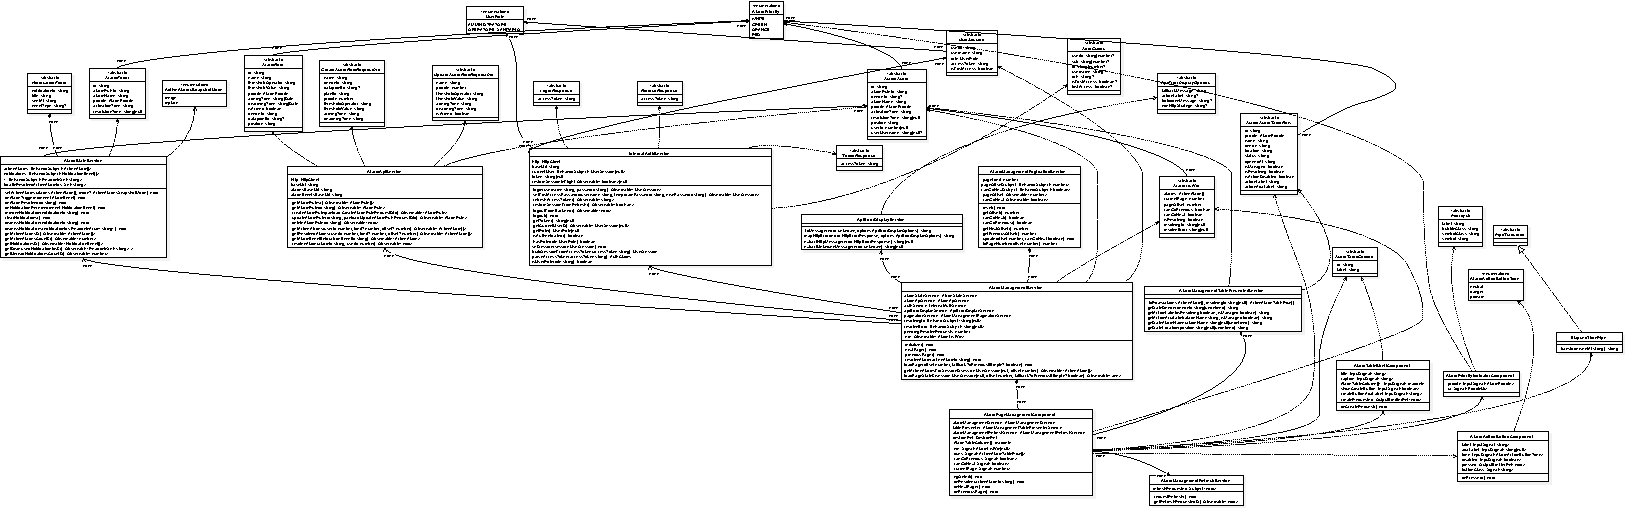
\includegraphics[width=\textwidth]{./frontend/alarm-management/alarm-management.pdf}
\captionof{figure}{\href{https://snakebyteteam.github.io/3-PB/Documenti_esterni/Specifica_tecnica/frontend/alarm-management/alarm-management.pdf}{Diagramma delle classi del modulo Alarm-management}}
\end{center}

\addAtr{-}{alarmManagementService: AlarmManagementService}{Servizio utilizzato per la gestione degli allarmi, incluse inizializzazione, risoluzione e navigazione tra le pagine.}
\addAtr{-}{tablePresenter: AlarmManagementTablePresenterService}{Servizio utilizzato per trasformare i dati degli allarmi nelle righe della tabella da visualizzare.}
\addAtr{-}{alarmManagementRefreshService: AlarmManagementRefreshService}{Servizio utilizzato per ricevere le notifiche di aggiornamento della lista allarmi.}
\addAtr{-}{destroyRef: DestroyRef}{Riferimento al ciclo di vita del componente, utilizzato per la cancellazione automatica delle sottoscrizioni.}
\addAtr{+}{columns: readonly AlarmTableColumn[]}{Lista delle colonne della tabella allarmi con i relativi identificativi ed etichette.}
\addAtr{+}{vm: Signal$<$AlarmListVm $|$ null$>$}{Segnale derivato dallo stream del view model del servizio di gestione allarmi.}
\addAtr{+}{rows: Signal$<$AlarmTableRow[]$>$}{Segnale calcolato che trasforma il view model corrente nelle righe della tabella tramite il presenter.}
\addAtr{+}{canGoPrevious: Signal$<$boolean$>$}{Segnale calcolato che indica se è possibile navigare alla pagina precedente.}
\addAtr{+}{canGoNext: Signal$<$boolean$>$}{Segnale calcolato che indica se è possibile navigare alla pagina successiva.}
\addAtr{+}{currentPage: Signal$<$number$>$}{Segnale calcolato che restituisce il numero della pagina corrente.}
\addMet{+}{ngOnInit() : void}{Inizializza il servizio di gestione allarmi e sottoscrive le notifiche di refresh per reinizializzare i dati.}
\addMet{+}{onResolve(activeAlarmId: string) : void}{Delega al servizio di gestione la risoluzione dell'allarme con l'identificativo specificato.}
\addMet{+}{onNextPage() : void}{Delega al servizio di gestione la navigazione alla pagina successiva degli allarmi.}
\addMet{+}{onPreviousPage() : void}{Delega al servizio di gestione la navigazione alla pagina precedente degli allarmi.}
\makeCl{AlarmPageManagementComponent}{Componente Angular che rappresenta la pagina di gestione degli allarmi attivi, con supporto alla paginazione e alla risoluzione. Si aggiorna automaticamente in risposta alle notifiche di refresh provenienti dal servizio dedicato.}

\addAtr{+}{id: string}{}
\addAtr{+}{priority: AlarmPriority}{}
\addAtr{+}{name: string}{}
\addAtr{+}{device: string}{}
\addAtr{+}{location: string}{}
\addAtr{+}{status: string}{}
\addAtr{+}{openedAt: string}{}
\addAtr{+}{isManaged: boolean}{}
\addAtr{+}{isResolving: boolean}{}
\addAtr{+}{isActionDisabled: boolean}{}
\addAtr{+}{actionLabel: string}{}
\addAtr{+}{actionAriaLabel: string}{}
\makeCl{ActiveAlarmTableRow}{Tipo che rappresenta una riga della tabella degli allarmi attivi. Raccoglie le informazioni di priorità, posizione, stato e i flag necessari alla gestione dell'azione di risoluzione.}

\addAtr{+}{alarms: ActiveAlarm[]}{}
\addAtr{+}{currentPage: number}{}
\addAtr{+}{pageOffset: number}{}
\addAtr{+}{canGoPrevious: boolean}{}
\addAtr{+}{canGoNext: boolean}{}
\addAtr{+}{isResolving: boolean}{}
\addAtr{+}{resolvingId: string $|$ null}{}
\addAtr{+}{resolveError: string $|$ null}{}
\makeCl{AlarmListVm}{Interfaccia che rappresenta il view model della lista degli allarmi attivi, contenente i dati della pagina corrente, lo stato di paginazione e le informazioni sull'eventuale risoluzione in corso.}

\addAtr{+}{pageLimit: number}{Numero massimo di allarmi visualizzabili per pagina.}
\addAtr{-}{pageOffsetSubject: BehaviorSubject$<$number$>$}{Subject che mantiene e notifica l'offset corrente della paginazione.}
\addAtr{-}{canGoNextSubject: BehaviorSubject$<$boolean$>$}{Subject che mantiene e notifica la disponibilità di una pagina successiva.}
\addAtr{+}{pageOffset\$: Observable$<$number$>$}{Stream reattivo che emette l'offset corrente della paginazione.}
\addAtr{+}{canGoNext\$: Observable$<$boolean$>$}{Stream reattivo che emette la disponibilità di una pagina successiva.}
\addMet{+}{reset() : void}{Reimposta l'offset a zero e la disponibilità della pagina successiva a false.}
\addMet{+}{getOffset() : number}{Restituisce il valore corrente dell'offset di paginazione.}
\addMet{+}{canGoNext() : boolean}{Restituisce true se è disponibile una pagina successiva.}
\addMet{+}{canGoPrevious() : boolean}{Restituisce true se l'offset corrente è maggiore di zero, indicando la presenza di una pagina precedente.}
\addMet{+}{getNextOffset() : number}{Calcola e restituisce l'offset della pagina successiva.}
\addMet{+}{getPreviousOffset() : number}{Calcola e restituisce l'offset della pagina precedente, con un minimo di zero.}
\addMet{+}{update(offset: number, canGoNext: boolean) : void}{Aggiorna l'offset corrente e la disponibilità della pagina successiva.}
\addMet{+}{toPageNumber(offset: number) : number}{Converte un offset nel corrispondente numero di pagina a partire da uno.}
\makeCl{AlarmManagementPaginationService}{Servizio Angular per la gestione dello stato di paginazione della lista allarmi. Espone stream reattivi e metodi di utilità per il calcolo degli offset e la navigazione tra le pagine.}

\addMet{+}{toRows(alarms: ActiveAlarm[], resolvingId: string $|$ null) : ActiveAlarmTableRow[]}{Trasforma una lista di allarmi attivi nelle corrispondenti righe della tabella, calcolando stato, etichette e flag di interazione.}
\addMet{-}{getSafeDevice(deviceId: string $|$ undefined) : string}{Restituisce l'identificativo del dispositivo normalizzato, o un trattino se assente o vuoto.}
\addMet{-}{getActionLabel(isResolving: boolean, isManaged: boolean) : string}{Restituisce l'etichetta del pulsante di azione in base allo stato di risoluzione e gestione dell'allarme.}
\addMet{-}{getActionAriaLabel(alarmName: string, isManaged: boolean) : string}{Restituisce l'etichetta aria del pulsante di azione per l'accessibilità, differenziando tra allarme già gestito e da gestire.}
\addMet{-}{getSafeAlarmName(alarmName: string $|$ null $|$ undefined) : string}{Restituisce il nome dell'allarme normalizzato, o la stringa senza nome se assente o vuoto.}
\addMet{-}{getSafeLocation(position: string $|$ null $|$ undefined) : string}{Restituisce la posizione dell'allarme normalizzata, o un trattino se assente o vuota.}


\makeCl{AlarmManagementTablePresenterService}{Servizio Angular che si occupa della trasformazione dei dati degli allarmi attivi nelle righe del modello di presentazione della tabella. Gestisce la normalizzazione dei valori e il calcolo delle etichette e dei flag di stato per ciascuna riga.}

\addAtr{-}{alarmStateService: AlarmStateService}{Servizio utilizzato per la gestione dello stato degli allarmi attivi in memoria.}
\addAtr{-}{alarmApiService: AlarmApiService}{Servizio utilizzato per le chiamate API relative agli allarmi.}
\addAtr{-}{authService: InternalAuthService}{Servizio di autenticazione utilizzato per recuperare l'utente corrente.}
\addAtr{-}{apiErrorDisplayService: ApiErrorDisplayService}{Servizio utilizzato per la formattazione dei messaggi di errore provenienti dalle API.}
\addAtr{-}{paginationService: AlarmManagementPaginationService}{Servizio utilizzato per la gestione dello stato di paginazione della lista allarmi.}
\addAtr{-}{resolvingId\$: BehaviorSubject$<$string $|$ null$>$}{Subject che mantiene l'identificativo dell'allarme attualmente in fase di risoluzione.}
\addAtr{-}{resolveError\$: BehaviorSubject$<$string $|$ null$>$}{Subject che mantiene il messaggio di errore relativo all'ultima operazione fallita.}
\addAtr{-}{pendingResolveRequests: number}{Contatore delle richieste di risoluzione allarme attualmente in corso.}
\addAtr{+}{vm\$: Observable$<$AlarmListVm$>$}{Stream reattivo che combina lo stato degli allarmi, la paginazione e gli errori in un unico view model.}
\addMet{+}{initialize() : void}{Reimposta la paginazione e carica la prima pagina degli allarmi attivi.}
\addMet{+}{nextPage() : void}{Carica la pagina successiva degli allarmi se disponibile.}
\addMet{+}{previousPage() : void}{Carica la pagina precedente degli allarmi se disponibile.}
\addMet{+}{resolveAlarm(activeAlarmId: string) : void}{Avvia la risoluzione dell'allarme specificato, aggiornando lo stato e ricaricando la pagina corrente al termine.}
\addMet{-}{loadPage(offset: number, fallbackToPreviousIfEmpty: boolean) : void}{Carica la pagina di allarmi corrispondente all'offset specificato, con fallback alla pagina precedente se la pagina risulta vuota.}
\addMet{-}{getActiveAlarmsForSession\$(session: UserSession $|$ null, offset: number) : \\ Observable$<$ActiveAlarm[]$>$}{Recupera gli allarmi attivi per la sessione utente corrente all'offset specificato, lanciando un errore se l'utente non è valido.}
\addMet{-}{loadPageState\$(session: UserSession $|$ null, offset: number, fallbackToPreviousIfEmpty: boolean) : Observable$<$\{alarms: ActiveAlarm[], pageOffset: number, \\ canGoNext: boolean\}$>$}{Calcola lo stato completo della pagina da caricare, gestendo il fallback alla pagina precedente e la verifica della disponibilità della pagina successiva.}
\makeCl{AlarmManagementService}{Servizio Angular per la gestione degli allarmi attivi, che coordina il caricamento paginato, la risoluzione e l'aggiornamento del view model reattivo. Integra i servizi di stato, API, autenticazione e paginazione per esporre un unico stream di dati ai componenti.}